
%(BEGIN_QUESTION)
% Copyright 2015, Tony R. Kuphaldt, released under the Creative Commons Attribution License (v 1.0)
% This means you may do almost anything with this work of mine, so long as you give me proper credit

\noindent
{\bf Lab Exercise -- introduction}

\vskip 5pt

Your team's task is to construct a system controlled by a PLC.  The system you choose to build shall use (at minimum) discrete input(s), discrete output(s), and either counter or timer functions.  This system will be expanded during the next course to include a three-pole contactor, so designing the system with this in mind (or simply installing the contactor in this exercise) will save you time later.  Project ideas include:

\begin{itemize}
\item{} Air compressor control, with high and low air pressure switches
\vskip 5pt
\item{} Water sump pump control, with high and low water level switches
\vskip 5pt
\item{} Other alternatives? {\it Must be pre-approved by instructor!}
\end{itemize}

In addition to functioning properly, the PLC program must be {\it fully} documented and edited for cleanliness and good programming form.  This includes labels (aliases, or symbolic names) for all inputs and outputs, and comments for each and every rung of logic explaining the rungs' functions.  Although there will be only one program submitted by each team, completion of this objective is individual, with each student explaining (at least) a part of the PLC program to the instructor.

\vskip 10pt

\underbar{Objective completion table:}

% No blank lines allowed between lines of an \halign structure!
% I use comments (%) instead, so that TeX doesn't choke.

$$\vbox{\offinterlineskip
\halign{\strut
\vrule \quad\hfil # \ \hfil & 
\vrule \quad\hfil # \ \hfil & 
\vrule \quad\hfil # \ \hfil & 
\vrule \quad\hfil # \ \hfil & 
\vrule \quad\hfil # \ \hfil & 
\vrule \quad\hfil # \ \hfil & 
\vrule \quad\hfil # \ \hfil \vrule \cr
\noalign{\hrule}
%
% First row
{\bf Performance objective} & {\bf Grading} & {\bf 1} & {\bf 2} & {\bf 3} & {\bf 4} & {\bf Team} \cr
%
\noalign{\hrule}
%
% Another row
Team meeting and prototype sketch (do {\it first!}) & mastery & -- & -- & -- & -- & \cr
%
\noalign{\hrule}
%
% Another row
Circuit design challenge & mastery & & & & & -- -- -- -- \cr
%
\noalign{\hrule}
%
% Another row
Complete I/O list & mastery & -- & -- & -- & -- & \cr
%
\noalign{\hrule}
%
% Another row
Prototype PLC program ({\it before programming!}) & mastery & -- & -- & -- & -- & \cr
%
\noalign{\hrule}
%
% Another row
Final wiring diagram and system inspection & mastery & & & & & -- -- -- -- \cr
%
\noalign{\hrule}
%
% Another row
Demonstration of working system & mastery & -- & -- & -- & -- & \cr
%
\noalign{\hrule}
%
% Another row
Final PLC program inspection & mastery &  &  &  &  & -- -- -- --  \cr
%
\noalign{\hrule}
%
% Another row
Lab question: Wiring connections & proportional &  &  &  &  & -- -- -- -- \cr
%
\noalign{\hrule}
%
% Another row
Lab question: Commissioning & proportional &  &  &  &  & -- -- -- -- \cr
%
\noalign{\hrule}
%
% Another row
Lab question: Mental math & proportional &  &  &  &  & -- -- -- -- \cr
%
\noalign{\hrule}
%
% Another row
Lab question: Diagnostics & proportional &  &  &  &  & -- -- -- -- \cr
%
\noalign{\hrule}
} % End of \halign 
}$$ % End of \vbox

The only ``proportional'' scoring in this activity are the lab questions, which are answered by each student individually.  A listing of potential lab questions are shown at the end of this worksheet question.  The lab questions are intended to guide your labwork as much as they are intended to measure your comprehension, and as such the instructor may ask these questions of your team day by day, rather than all at once (on a single day).

\vskip 10pt

{\bf It is essential that your team plans ahead what to accomplish each day.  A short (10 minute) team meeting at the beginning of each lab session is a good way to do this, reviewing what's already been done, what's left to do, and what assessments you should be ready for.  There is a lot of work involved with building, documenting, and troubleshooting these working instrument systems!}

As you and your team work on this system, you will invariably encounter problems.  You should always attempt to solve these problems as a team before requesting instructor assistance.  If you still require instructor assistance, write your team's color on the lab whiteboard with a brief description of what you need help on.  The instructor will meet with each team in order they appear on the whiteboard to address these problems.





\vfil \eject

\noindent
{\bf Lab Exercise -- team meeting and prototype sketch}

\vskip 5pt

An important first step in completing this lab exercise is to {\bf meet with your instructor} as a team to discuss safety concerns, team performance, and specific roles for team members.  If you would like to emphasize exposure to certain equipment (e.g. use a particular type of control system, certain power tools), techniques (e.g. fabrication), or tasks to improve your skill set, this is the time to make requests of your team so that your learning during this project will be maximized.

\vskip 10pt

An absolutely essential step in completing this lab exercise is to work together as a team to {\bf sketch a prototype diagram} showing what you intend to build.  This usually takes the form of a simple electrical schematic and/or loop diagram showing all electrical connections between components, as well as any tubing or piping for fluids.  This prototype sketch need not be exhaustive in detail, but it does need to show enough detail for the instructor to determine if all components will be correctly connected for their safe function.

For example, if you intend to connect field devices to a PLC (Programmable Logic Controller), your prototype sketch must show how those devices will connect to typical input/output terminals on the PLC, where electrical power will be supplied, etc.  Prototype sketches need not show all intermediary connections between components, such as terminal blocks in junction boxes between the field device and the controller.

You should practice good problem-solving techniques when creating your prototype sketch, such as consulting equipment manuals for information on component functions and marking directions of electric current, voltage polarities, and identifying electrical sources/loads.  Use this task as an opportunity to strengthen your analytical skills!  Remember that you will be challenged in this program to do all of this on your own (during ``capstone'' assessments), so do not make the mistake of relying on your teammates to figure this out for you -- instead, treat this as a problem {\it you} must solve and compare your results with those of your teammates.

Your team's prototype sketch is so important that the instructor will demand you provide this plan before any construction on your team's working system begins.  {\it Any team found constructing their system without a verified plan will be ordered to cease construction and not resume until a prototype plan has been drafted and approved!}  Similarly, you should not deviate from the prototype design without instructor approval, to ensure nothing will be done to harm equipment by way of incorrect connections.  Each member on the team should have ready access to this plan (ideally possessing their own copy of the plan) throughout the construction process.  Prototype design sketching is a skill and a habit you should cultivate in school and take with you in your new career.

\vskip 10pt

Select a PLC with modular (add-on) I/O cards to provide sufficient complexity for the project.  Monolithic ``brick'' PLCs (with no add-on I/O modules) are not acceptable for this project.  An Allen-Bradley SLC 500 PLC would be a good choice, as well as a Siemens S7 series or an AutomationDirect Productivity 3000.

You will also need to select appropriate field devices (switches, pumps, etc.) for your project.  You are free to use the field devices left over from the relay-based motor control lab if you prefer.

The next step should be finding appropriate documentation for your PLC.  All PLC manufacturers provide manuals and datasheets for their products online.  Use this documentation to identify how to properly wire, power, and program your team's PLC.  

PLC equipment manuals always provide sample diagrams showing how external components may connect to the I/O points.  Feel free to use these sample diagrams as templates for your prototype sketch.  {\it This is the most challenging portion of your wiring, so be sure to work with your teammates to get this right!}

\vskip 10pt

{\bf Planning a functioning system should take no more than a couple of hours if the team is working efficiently, and will save you hours of frustration (and possible component destruction!).}







\vfil \eject

\noindent
{\bf Lab Exercise -- circuit design challenge}

\vskip 5pt

Connect an ``ice cube'' relay to one of the outputs on a PLC, so that the PLC can control the energization of the relay.  All electrical connections must be made using a terminal strip (no twisted wires, crimp splices, wire nuts, spring clips, or ``alligator'' clips permitted).  Program this PLC to implement a motor start/stop (latching) control function.  {\it In order to ensure your program has not been pre-written in your computer prior to this assessment, you will be asked to sketch a correct ladder-diagram PLC program on paper to implement this function prior to using a computer.}

You must connect a ``commutating'' diode in parallel with the relay's coil to prevent the phenomenon known as ``inductive kickback,'' which may otherwise damage the transistor output on a PLC.  Note that incorrectly connecting this diode will present a short-circuit to the PLC, so you {\it must} get it right!

This exercise tests your ability to properly interpret the ``pinout'' of an electromechanical relay, properly wire a PLC output channel to control a relay's coil, properly polarize a commutating diode to prevent inductive kickback from damaging the PLC output, and use a terminal strip to organize all electrical connections.  It also tests your ability to program motor start/stop logic using either a seal-in contact or latching (retentive) coil instructions.

$$\includegraphics[width=15.5cm]{i03655x01.eps}$$

\vskip 10pt

The following components and materials will be available to you: assorted ``ice cube'' {\bf relays} with DC-rated coils and matching {\bf sockets} ; {\bf terminal strips} ; 1N400X rectifying {\bf diodes} ; lengths of {\bf hook-up wire}.  You will be expected to supply your own screwdrivers and multimeter for assembling and testing the circuit at your desk.  

\vskip 20pt

\noindent
{\bf ``Start'' switch to input}: \underbar{\hskip 20pt} \hskip 30pt {\bf ``Stop'' switch to input}: \underbar{\hskip 20pt} \hskip 30pt {\bf Relay to output}: \underbar{\hskip 20pt}

\vskip 20pt

\noindent
{\bf PLC program} (instructor chooses): \hskip 20pt \underbar{\hskip 20pt} Seal-in contact \hskip 20pt \underbar{\hskip 20pt} Retentive coils



\vfil







\vfil \eject

\noindent
{\bf Lab Exercise -- developing a PLC I/O list}

\vskip 5pt

It is a good idea when programming any computer system to first identify all the input and output signals to the system, as well as internal variables if possible, before commencing on the development of the program itself.  In order to reinforce this practice, your team will be required to develop a complete list of all input and output points on your proposed system along with any tagnames (also known as ``symbols'' or ``nicknames'') identifying the function of each.

Once this list is complete and you are ready to begin developing the PLC program, you can enter all the tagnames and define the I/O points as your very first programming step.  With this data in place, the writing of your program will be made easier because each I/O tag you reference will already be defined and labeled, reminding you of their functions within the system.

\vskip 10pt

Here is a sample I/O list for a motor control PLC program:

% No blank lines allowed between lines of an \halign structure!
% I use comments (%) instead, so that TeX doesn't choke.

$$\vbox{\offinterlineskip
\halign{\strut
\vrule \quad\hfil # \ \hfil & 
\vrule \quad\hfil # \ \hfil & 
\vrule \quad\hfil # \ \hfil & 
\vrule \quad\hfil # \ \hfil \vrule \cr
\noalign{\hrule}
%
% First row
{\bf Hardware I/O terminal} & {\bf I/O type} & {\bf Tagname} & {\bf Notes} \cr
%
\noalign{\hrule}
%
% Another row
Card 1, terminal IN0 & 24 VDC discrete input & {\tt START\_PB} & Black pushbutton, \cr
 &  &  & momentary NO contacts \cr
%
\noalign{\hrule}
%
% Another row
Card 1, terminal IN1 & 24 VDC discrete input & {\tt STOP\_PB} & Red pushbutton, \cr
 &  &  & momentary NC contacts \cr
%
\noalign{\hrule}
%
% Another row
Card 1, terminal IN2 & 24 VDC discrete input & {\tt E\_STOP} & Red pushbutton, \cr
 &  &  & latching NC contacts \cr
%
\noalign{\hrule}
%
% Another row
Card 2, terminal IN0 & 4-20 mA analog input & {\tt MTR\_TEMP} & Current signal scaled \cr
 &  &  & 0 to 150 deg F \cr
%
\noalign{\hrule}
%
% Another row
Card 3, terminal OUT0 & 120 VAC discrete output & {\tt CONTACTOR} & To terminal A1 \cr
%
\noalign{\hrule}
} % End of \halign 
}$$ % End of \vbox








\vfil \eject

\noindent
{\bf Lab Exercise -- wiring the system}

\vskip 5pt

The Instrumentation lab is set up to facilitate the construction of working systems, with over a dozen junction boxes, pre-pulled signal cables, and ``racks'' set up with 2-inch vertical pipes for mounting instruments.  The only wires you should need to install to build a working system are those connecting the field instrument to the nearest junction box, and then small ``jumper'' cables connecting different pre-installed cables together within intermediate junction boxes.

Your team's PLC must be installed in a suitable electrical enclosure, with AC power fed to it through a fuse or circuit breaker (on the ``hot'' conductor only), and firmly grounded (the ground conductor of the power cord securely fastened to the metal frame of the enclosure and the PLC chassis).

All I/O wiring should be neatly loomed together and/or run through wire duct (``Panduit'').  Power to I/O cards must be routed through their own fuses so that I/O power may be disconnected independently of power to the PLC processor and rack.

\vskip 10pt

{\bf Common mistakes:}

\begin{itemize}
\item{} Neglecting to consult the manufacturer's documentation for field instruments (e.g. how to wire them, how to calibrate them).
\item{} Proceeding with wiring {\it before} creating an initial sketch of the circuitry and checking that sketch for errors.
\item{} Mounting the field instrument(s) in awkward positions, making it difficult to reach connection terminals or to remove covers when installed.
%\item{} Improper pipe/tube fitting installation (e.g. trying to thread tube fittings into pipe fittings and vice-versa).
\item{} Failing to tug on each and every wire where it terminates to ensure a mechanically sound connection.
\item{} Students working on portions of the system in isolation, not sharing with their teammates what they did and how.  It is important that the whole team learns all aspects of their system!
\end{itemize}

\vskip 10pt

{\bf Building a functioning system should take no more than one full lab session (3 hours) if all components are readily available and the team is working efficiently!}




\vfil \eject

\noindent
{\bf Lab Exercise -- programming the system}

\vskip 5pt

Like wiring a control system, programming one is best done with thoughtful planning rather than a ``design-as-you-build'' approach.  Each team will work with the instructor to develop a ``prototype'' PLC program, usually on a whiteboard or on paper.  {\it Having multiple teams prototype their programs on whiteboards within the same classroom works well to foster peer review of programming, where teams analyze and critique other teams' programming solutions!}  Your prototype program should completely address the following points:

\begin{itemize}
\item{} Identify all inputs to the PLC, giving each one a sensible tagname
\item{} Identify all signal outputs from the PLC, giving each one a sensible tagname
\item{} Identify all major program functions (i.e. {\it What must this program do?})
\item{} Identify all internal variables necessary for these functions, giving each one a sensible tagname
\item{} Identify all system variables necessary for these functions (e.g. real-time clock/calendar variables)
\end{itemize}

The importance of identifying and naming all relevant variables is paramount to ``clean'' programming.  This is especially true when an HMI (Human-Machine Interface) is to be connected to the PLC, and all relevant variables must be named there as well.

A reasonable approach to developing a robust program prototype is to create your prototype in your own personal (``brick'') PLC, de-bugging it there with all the switches in place to simulate input signals.  Even if your personal PLC is a different model (or manufacture) than the project PLC, this is a very helpful exercise.  Furthermore, it allows you to continue program development outside of school when you do not have access to the project PLC.

\vskip 10pt

Only after a prototype program is developed should you begin programming the project PLC.  I recommend the following steps:

\begin{itemize}
\item{} Establish communications between PLC and personal computer (PC)
\item{} Connect all I/O cards (modules) to the PLC and get them recognized by the processor
\item{} Assign tagnames to all relevant variables, beginning with I/O points
\item{} Enter a simplified version of the program, running to check for ``bugs''
\item{} Diagnose any program problems
\item{} Add complexity to the program (e.g. additional features) and run to check for ``bugs''
\item{} Repeat last two steps as often as necessary
\item{} Add comments to each and every line of the program, explaining how it functions
\end{itemize}

The final program should be well-documented, clean, and as simple as possible.  All members of the team should have a hand in designing the program, and everyone {\it must} thoroughly understand how it works.

\vskip 10pt

{\bf Common mistakes:}

\begin{itemize}
\item{} Waiting too long after writing the program code to insert comments.  This is best done immediately, while everything makes sense and is fresh in your memory!
\item{} Insufficient commenting -- only makes sense to the person who did the programming
\item{} Students working on portions of the program in isolation, not sharing with their teammates what they did and how.  It is important that the whole team learns all aspects of their system!
\end{itemize}








\vfil \eject

\noindent
{\bf Lab Exercise -- documenting the system}

\vskip 5pt

Each student must sketch their own {\it wiring diagram} for their team's system, following industry-standard conventions.  Sample diagrams for input and output wiring are shown in the next question in this worksheet.  These wiring diagrams must be {\it comprehensive} and {\it detailed}, showing every connection, every cable, every terminal block, etc.  The principle to keep in mind here is to make the wiring diagram so complete and unambiguous that anyone can follow it to see what connects to what, even someone unfamiliar with industrial instrumentation.  In industry, control systems are often constructed by contract personnel with limited understanding of how the system is supposed to function.  The associated diagrams they follow must be so complete that they will be able to connect everything properly without necessarily understanding how it is supposed to work.

When your entire team is finished drafting your individual wiring diagrams, call the instructor to do an inspection of the system.  Here, the instructor will have students take turns going through the entire system, with the other students checking their diagrams for errors and omissions along the way.  During this time the instructor will also inspect the quality of the installation, identifying problems such as frayed wires, improperly crimped terminals, poor cable routing, missing labels, lack of wire duct covers, etc.  The team must correct all identified errors in order to receive credit for their system.  

After successfully passing the inspection, each team member needs to place their wiring diagram in the diagram holder located in the middle of the lab behind the main control panel.  When it comes time to troubleshoot another team's system, this is where you will go to find a wiring diagram for that system!

\vskip 10pt

{\bf Common mistakes:}

\begin{itemize}
\item{} Forgetting to label all signal wires (see example wiring diagrams).
\item{} Forgetting to label all field instruments with their own tag names (e.g. PSL-83).
\item{} Forgetting to note all wire colors.
\item{} Forgetting to put your name on the wiring diagram!
\item{} Basing your diagram off of a team-mate's diagram, rather than closely inspecting the system for yourself.
\end{itemize}

\vskip 10pt

{\bf Creating and inspecting accurate wiring diagrams should take no more than one full lab session (3 hours) if the team is working efficiently!}







\vfil \eject

\noindent
{\bf Lab questions}

\begin{itemize}
\item{} {\bf Wiring connections}
\item{} Determine correct wire connections between field components and a PLC I/O card to create a working PLC input or output circuit, based on diagrams of components with terminals labeled
\item{} Correctly determine all electrical sources and loads, as well as all voltage polarities and current directions, in a DC input or output circuit, based on diagrams of field components and the PLC's I/O card with terminals labeled
\end{itemize}

\filbreak

\begin{itemize}
\item{} {\bf Commissioning and Documentation}
\item{} Explain what is meant by the term ``sinking'' with regard to a PLC input card (DC)
\item{} Explain what is meant by the term ``sourcing'' with regard to a PLC input card (DC)
\item{} Explain what is meant by the term ``sinking'' with regard to a PLC output card (DC)
\item{} Explain what is meant by the term ``sourcing'' with regard to a PLC output card (DC)
\item{} Explain what a ``TRIAC'' PLC output card is, and how it differs from DC output cards
\item{} Explain what a ``relay'' PLC output card is, and how it differs from sourcing or sinking DC output cards
\item{} Explain the distinction between ``online'' and ``offline'' programming modes for a PLC
\end{itemize}

\filbreak

\begin{itemize}
\item{} {\bf Mental math} (no calculator allowed!)
\item{} Convert a binary number into decimal
\item{} Convert a binary number into hexadecimal
\item{} Convert a decimal number into binary
\item{} Convert a hexadecimal number into binary
\item{} Convert a hexadecimal number into decimal
\end{itemize}

\filbreak

\begin{itemize}
\item{} {\bf Diagnostics}
\item{} Examine a PLC program and identify any mistakes in it
\item{} Determine whether or not a given diagnostic test will provide useful information, given a set of symptoms exhibited by a failed system
\item{} Identify at least two plausible faults given the results of a diagnostic test and a set of symptoms exhibited by a failed system
\item{} Propose a diagnostic test for troubleshooting a failed system and then explain the meanings of two different test results
\end{itemize}


\vfil \eject

\noindent
{\bf Wiring diagram requirements}

\begin{itemize}
\item{} {\bf Wiring diagram}
\item{} Proper symbols and designations used for all components.
\item{} Relay coil and contacts properly named.
\end{itemize}

\begin{itemize}
\item{} {\bf Text descriptions}
\item{} Each instrument documented below (tag number, description, etc.).
\item{} Calibration (input and output ranges) given for each instrument, as applicable.
\end{itemize}

\begin{itemize}
\item{} {\bf Connection points}
\item{} All terminal blocks properly labeled.
\item{} All terminals shown in proper order on diagram.
\item{} All I/O cards and points fully labeled (complete with program addresses).
\item{} All wires are numbered.
\item{} All electrically-common points in the circuit shall bear the same wire number.
\item{} All wire colors shown next to each terminal.
\end{itemize}

\begin{itemize}
\item{} {\bf Cables and tubes}
\item{} Multi-pair cables or pneumatic tube bundles going between junction boxes and/or panels need to have unique numbers (e.g. ``Cable 10'') as well as numbers for each pair (e.g. ``Pair 1,'' ``Pair 2,'' etc.).
\end{itemize}

\begin{itemize}
\item{} {\bf Energy sources}
\item{} All power source intensities labeled (e.g. ``24 VDC,'' ``120 VAC,'' ``20 PSI'')
\item{} All shutoff points labeled (e.g. ``Breaker \#5,'' ``Valve \#7'')
\end{itemize}

\underbar{file i03655}
%(END_QUESTION)





%(BEGIN_ANSWER)


%(END_ANSWER)





%(BEGIN_NOTES)

\noindent
{\bf Wiring diagrams / inspections:}

I strongly recommend checking off students' wiring diagrams while you inspect their circuit (checking for secure wiring, proper tubing, good conduit installation, etc.) with them.  Have all team members take you on a ``tour'' of their completed system, with each team member explaining a different portion of the circuit you select while using their own wiring diagram as a guide.  While a student is explaining their section of the system, you can check the other students' wiring diagrams for accuracy.  This not only saves time by consolidating the tasks of system inspection and wiring diagram verification, but it also ensures students can actually relate their wiring diagrams to the system they have built and articulate that understanding to you.

\vskip 10pt

\goodbreak

\noindent
{\bf Troubleshooting fault ideas:}

\medskip
\goodbreak
\item{} Strip wire at terminal, then insert insulated wire end under terminal and tighten (open wire fault)
\item{} Cut signal cable somewhere in mid-conduit (open wire fault)
\item{} Push a thumbtack through the cable somewhere in mid-conduit (shorted wire fault)
\item{} Wire instrument cable conductors backward (construction fault)
\item{} Plug air tube connections using portion of foam earplug stuffed into tube fitting (slow response fault)
\end{itemize}










\vfil \eject

\noindent
{\bf Lab questions}

\vskip 20pt

\item{$(1)$} Correctly determine all voltage polarities and current directions in the {\tt Q0.0} output circuit of this Siemens PLC (i.e. circuit powering the LED):

$$\includegraphics[width=15.5cm]{i03655x02.eps}$$

\vskip 20pt

\item{$(2)$} Explain the difference between ``online'' and ``offline'' modes in the PLC programming software.

\vskip 20pt

\item{$(3)$} Convert the hexadecimal number {\tt 2AE} into decimal.

\vskip 20pt

\filbreak

\item{$(4)$} This motor refuses to start when the ``Start'' pushbutton is pressed.  Examining the PLC while pressing the ``Start'' switch, a technician notices that the LED indicators for input channels 0 and 2 are lit, but not the LED for input channel 4 or the LED for output channel 5.  This same technician suggests using a voltmeter to test for AC voltage between terminals {\tt VAC 2} and {\tt OUT 5} on the PLC's output card.  Identify whether this diagnostic test will provide information useful for pinpointing the fault in this system, being sure to explain why or why not:

$$\includegraphics[width=15.5cm]{i03655x03.eps}$$











\vfil \eject

\noindent
{\bf Lab questions}

\vskip 20pt

\item{$(1)$} Correctly determine all voltage polarities and current directions in the {\tt I0.1} input circuit of this Siemens PLC:

$$\includegraphics[width=15.5cm]{i03655x02.eps}$$

\vskip 20pt

\item{$(2)$} Explain what a ``TRIAC'' PLC output card is, and how it differs from DC output cards

\vskip 20pt

\item{$(3)$} Convert the decimal number {\tt 145} into hexadecimal.

\vskip 20pt

\filbreak

\item{$(4)$} This motor refuses to start when the ``Start'' pushbutton is pressed.  Examining the PLC while pressing the ``Start'' switch, a technician notices that the LED indicators for input channels 0 and 4 are lit, but not the LED for input channel 2 or the LED for output channel 5.  This same technician suggests using a voltmeter to test for AC voltage between terminals {\tt IN 2} and {\tt COM} on the PLC's input card.  Identify whether this diagnostic test will provide information useful for pinpointing the fault in this system, being sure to explain why or why not:

$$\includegraphics[width=15.5cm]{i03655x03.eps}$$

%INDEX% Lab exercise, motor control circuit (PLC-based)

%(END_NOTES)


